\chapter{Postlude}

`What happens if I turn it the other way?' my youngest daughter shouted in excitement as she pointed at the rotary dial on the new radio I had just picked up during our Stockholm vacation. She had just tested the `scratching' function of the Teenage Engineering OB-4, branded as a \emph{magic} radio. The `magic' part of the radio is the implementation of a synthesizer module into the device. A built-in continuous recording mode makes it possible to rewind whatever one listens to and adjust the playback speed. Instead of only listening passively to the radio, my daughters started modifying the sound. They quickly discovered how to create loops of various durations. I was equally excited about the ambiance mode, which makes a `sonic soup' of the incoming audio based on a long delay line. `What do you call such a thing' my wife asked, looking at me to get a straightforward answer. `Well, it is kind of\ldots kind of\ldots a musicking technology,' I replied, trying to come up with a better term than `magic' to describe its function. After all, there is nothing magical about the device. Instead, it is an excellent meeting point between creative art and sound engineering. `This device is in many ways a real-world example of the conclusion of my new book,' I added, trying to explain my thoughts on how new technologies allow for active musical experiences.

\section{Musicking technology}

As I have argued throughout this book, new technologies change the way we perform and perceive music. New instruments are developed every year. Most of them are never commercialized, and many that reach the market fail to make an impact. There is also much experimentation when it comes to music technologies targeted at music listening. Both types of technologies---targeted at performers or perceivers---challenge the traditional idea of what an instrument should be or function. They expand the action--sound palettes available, the spatiotemporal distance between instruments and performers, and the resultant musical output. Not least do they blur the lines between different actors. Today, many composers build instruments, record sounds, and perform themselves. Similarly, performers may spend more time programming sounds and musical structures before a performance than they do on stage. In parallel, perceivers get access to musical apps that let them create music on their own or modify pre-recorded music. In many ways, the processes of making and experiencing music are changing.

New musicking technologies have a different scope and intention than traditional music technologies. Today's new instruments are not only sound-makers; they are often also music-makers with much embedded musical knowledge. In some cases, the instrument may contain a more or less fixed piece of music or artificial intelligence that can create music on the fly. Other times, a musicking technology may allow for full musical exploration or tweaking of the sonic output in the case of the magic radio. The development of such devices is escalating. However, as I have argued in earlier chapters, the shift from sound-makers to music-makers began centuries ago. The church organ made it possible to change the sound's timbre and play harmonic tones. Music boxes embedded whole compositions that could be played back at different speeds. The shift from sound-makers to music-makers happened long before electricity came into play.

`Children should play the piano, not on a mobile phone,' a parent once told me when I talked about my research. Fortunately, I do not think that new musicking technologies need to overthrow other musical activities. My daughters play with all the new electro-acoustic instruments I bring home. They also enjoy playing trombone, saxophone, flute, and piano. All these instruments allow for different sonic and musical experiences, and they can perfectly well co-exist. People still play acoustic instruments even though electro-acoustic instruments have been available for decades. I am not afraid that devices like the magic radio will lead to a decline in piano playing. However, new musicking technologies may allow for more active and embodied musical experiences. They may open for more playful musical engagement than only passively listening to the radio.

How should we think about musical instruments in the future? Should all the emerging musicking technologies be regarded as instruments? In many ways, trying to define an instrument may cause more harm than good. One could be conservative and say that an instrument should allow for real-time musicianship with a low action--sound separation. That would rule out most new devices. Instead, one could be liberal and argue that any musicking technology should be considered an instrument. Then one risks `watering out' the instrument concept to such an extent that nobody understands its purpose. The musicking quadrant can help in structuring our thoughts on the matter. As shown in Figure~\ref{fig:music-quadrant12}, new instruments may be thought of as bridging over between different musical functions, roles, and actors. What is clear is that a new `instrument' definition will cover more than only sound-makers. In my thinking, instruments need to allow for active and embodied musical interaction within a certain level of action--sound separation and spatiotemporal distance. There needs to be a musical \emph{inter}action. Thus defining instruments based on their techno-cognitive properties is more valuable than looking only at their technical construction.

\begin{figure}[tp]
  \centerline{
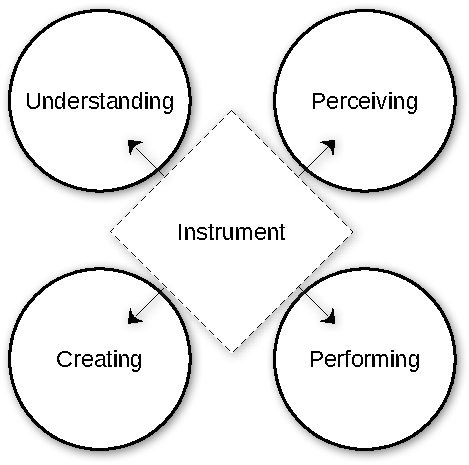
\includegraphics[width=.6\columnwidth]{figures/79-quadrant-crop.pdf}
\caption{New instruments challenge the traditional roles of the musicking quadrant.}
\label{fig:music-quadrant12}
}
\end{figure}


\section{Differences between couplings and mappings}

One of my core arguments has been that there are techno-cognitive differences between action--sound couplings and mappings. I introduced this distinction in my Ph.D. dissertation \citep{jensenius_actionsound_2007}, although the argument was not yet fully developed at the time. My focus on action--sound couplings was inspired by recent trends in embodied music cognition. `Ways of Listening' by Eric \citet{clarke_ways_2005} had just come out, and I had read a draft manuscript of `Embodied Music Cognition and Mediation Technology' by Marc \citet{leman_embodied_2008}. My clear-cut separation between the couplings of acoustic instruments and the mappings of electro-acoustic instruments was based on speculations about how our brains work. There is a growing body of neuroscientific research into relationships between action and sound in general. However, less is known about possible cognitive differences between action--sound couplings and mappings.

It should be possible to investigate some of these differences scientifically. For example, is there a difference in the way we perceive an acoustic and a digital piano? Such instruments may look and sound more or less the same. My hybrid piano feels almost the same as playing an acoustic grand piano. Still, I believe there are differences. For example, an acoustic instrument will almost always be slightly out of tune. However, the most significant conceptual difference is that one instrument runs on electricity. If the power is off, there is no sound. When I hit the key on an acoustic piano, it will always sound with a piano-like tone. When I press the key on an electro-acoustic piano, I never know what will happen. It may not sound if it is not turned on, the volume control is down, or the power is out. If it sounds, there is no way that I could have predicted its sonic qualities. This makes me approach acoustic and electro-acoustic instruments differently. The same is the case when others perform. My expectations are shaped by the instrument I see. If someone picks up the violin, I know more or less what to expect. If they sit with a laptop, I have no idea. Is that a problem? Not necessarily. Several of my strongest musical experiences have been with electro-acoustic instruments. But I have also experienced many unsuccessful performances with such instruments.

My attempt at separating acoustic and electro-acoustic instruments is not based on a wish to say that one is better than the other. Instead, I have created a theoretical framework that can help us understand more about musicking technologies, regardless of whether we are talking about a violin or a new electro-acoustic instrument. Hopefully, this can also help in discussing the qualities of various instruments. One could argue that this is primarily of theoretical interest. However, such questions become real when I sit on student entry committees in my department. It is not uncommon to compare one student playing classical music on a clarinet to another presenting a live electronics piece on a laptop. It is impossible to make informed judgments about such performances if we are not equipped with a vocabulary to describe the instruments in question and the different types of musicking that they afford. This book does not provide a solution for making such judgments. However, it can hopefully help in understanding more about different types of musicking.


\section{Diversity and accessibility}

Several topics have been left out or only marginally discussed in this book. My main story has focused on the individual's experience with instruments. In the future, it would be exciting to combine such a techno-cognitive perspective with \emph{socio-technical} theories, such as the one described by \citet{bijker_bicycles_1997}. A broader sociocultural perspective could have opened for discussing diversity more broadly. The male dominance of the music technology research field is well documented. \citet{xambo_who_2018} showed that only around 14\% of authors at the annual NIME conferences are women. This corresponds with the low female numbers found by \citet{born_music_2015} in a study of music technology education in the UK.
There are also few women in the music technology performance scene, as documented by \citet{gadir_forty-seven_2017} in studies of female DJs. Based on interviews with women experts in the field, \citet{jawad_how_2020} argues that the term `music technology' may in itself be problematic.

There are also other diversity issues in the music technology community.
\citet{frid_diverse_2019} has described the need for more focus on accessibility and inclusivity in musical interaction design. \citet{morreale_where_2021} has critized the neo-colonial tendencies of current music technologies. Finally, there has also been a widened understanding of the challenges with the `white racial frame’ that limits the topics, discurse, and job opportunities in music research more generally \citep{ewell_music_2020}. My approach is shaped through the `frame' of a white Northern-European male. Until recently, I did not explicitly focus on diversity or accessibility in my research. However, my growing awareness of these issues has influenced some of my choices when developing the theories presented in this book. I hope to make a difference by pushing the musicking technology concept and experimenting with building prototypes of such devices. I also hope that it helps (a little) to acknowledge the diversity challenges of the various fields I am involved in.


\section{Sustainability}

Sustainability is another topic that is quickly emerging based on the environmental crisis we are currently experiencing. I am generally optimistic about the possibilities of new technologies. For example, I believe that developing better solutions for telematic performance may help decrease the need to travel in the future. However, I am increasingly concerned about today's technological consumption, which is unsustainable. There has been a growing focus on sustainability in general human-computer interaction \citep{hazas_digital_2017, chapman_emotionally_2015}, but less so in the music (technology) research community. \citet{devine_decomposed_2019} talks about `petrocapitalism' in his study of the negative environmental impact of the music industry. Even though there are industries with larger impacts, that is no excuse for not making a change.

\citet{mankoff_environmental_2007} have argued that technology designers can contribute by keeping sustainability in mind when developing new products. This can be done from two perspectives:

\begin{itemize}
  \item Sustainability through design
  \item Sustainability in design
\end{itemize}

\citet[p. 204]{king_understanding_2016} exemplify sustainability through design with an innovative water dispenser. The dispenser has a built-in counter that lets the user know how many plastic bottles have been saved by using the machine. It is a small design inclusion but has a `game-like' effect when giving users positive feedback.
I have yet to come across a good example of a musical instrument focusing on sustainability through design. There are also, unfortunately, few examples of sustainability in design in the music technology community \citep{masu_nime_2021}. One example that comes to mind is the Fingerphone by \citet{freed_fingerphone_2012}. This project was based on recreating a popular instrument from the 1970s, the Stylophone, with a more sustainable technological implementation. His approach was based on \emph{reducing} the number of components in the device. He also \emph{reused} components from other devices, such as the built-in battery. Finally, he built a large part of the device with \emph{recyclable} paper, using principles by \citet{koehly_fabrication_2011}. Through these simple measures, Freed showed that it is possible to make a complete musical instrument with a relatively small environmental footprint.

I have several architect friends, and I hear many of them talk about the future of their profession being \emph{re}construction rather than construction. We should probably focus more on reconstruction also in the music technology community. Here we can learn from hardware hackers, experts in reusing and repurposing technologies for musical purposes \citep{collins_handmade_2020}. We can also build on the exisiting tradition of building and maintaining traditional musical insturments. Instruments have for centuries been built to last. It is only in recent years that consumer electronics have been designed to break. Thus creating with quality in mind is essential. `Designing for disassembly' is another \citep{crowther_design_2005}. That may help to fix broke instruments but also facilitate repurposing.

How can one get started with a more sustainable music technology practice? Table~\ref{tab:framework} shows a framework we proposed for considering the environmental cost of activities related to designing, building, and using instruments \citep{masu_nime_2021}. The matrix is not exhaustive but is a tool for considering one's environmental footprint. The columns represent the research stage. The first is the \emph{making} of an instrument, which covers design, construction, prototyping, and coding. Next is the \emph{testing} phase, including performances made as part of an iterative design phase. The \emph{using} phase covers regular rehearsals and performances. Finally, \emph{disposing} covers the end-of-life stages of an instrument. Five different topics can be considered for each step. The \emph{materials} are the physical parts necessary to build a device. The \emph{consumables} are physical parts that need to be regularly replaced, such as the reeds of wind instruments and markers of motion-capture-based instruments. \emph{Storage} covers the environmental cost of both physical and digital storage. \emph{Processing} is the cost of computing, which is mainly relevant for instruments built with CPU-intensive AI components. Finally, \emph{transport} covers all sorts of transportation related to the different phases, ranging from the transport of instrument parts to travel as part of performance activities.

\begin{table}[tp]
  \centerline{
  \begin{tabular}{|r|r|c|c|c|c|}
    \hline
  \multirow{2}{*}{} & \multirow{2}{*}{} & \multicolumn{4}{c|}{Research stage}\tabularnewline
  \cline{3-6} \cline{4-6} \cline{5-6} \cline{6-6}
   &  & Making & Testing & Using & Disposing\tabularnewline
  \hline
  \multirow{5}{*}{\rotatebox{90}{Resources}} & Materials &  &  &  & \tabularnewline
  \cline{2-6} \cline{3-6} \cline{4-6} \cline{5-6} \cline{6-6}
   & Consumables &  &  &  & \tabularnewline
  \cline{2-6} \cline{3-6} \cline{4-6} \cline{5-6} \cline{6-6}
   & Storage &  &  &  & \tabularnewline
  \cline{2-6} \cline{3-6} \cline{4-6} \cline{5-6} \cline{6-6}
   & Processing &  &  &  & \tabularnewline
  \cline{2-6} \cline{3-6} \cline{4-6} \cline{5-6} \cline{6-6}
   & Transport &  &  &  & \tabularnewline
   \hline
  \end{tabular}
}
  \caption{A framework for reflecting on the environmental impact of a musical instruments \citep{masu_nime_2021}. }
  \label{tab:framework}
\end{table}

We introduced the framework in a workshop at the NIME conference in 2021. The participants tried to fill out the matrix for one of their instruments. Many found it challenging to fill all the cells. Still, it was perceived as a valuable tool to help structure one's thoughts. Several argued that transportation---either their own or related to parts and equipments---is what drives their environmental cost the most. Some said they had not thought about the environmental cost of adding batteries to their instruments. Others started reflecting on the use of intensive machine learning for their sound engines. Personally, I started to think about the environmental footprint of keeping an extensive collection of instruments in physical storage. That storage space needs heating, and it could probably have been used for other things. It made me realize that I need to reduce the number of instruments I keep in storage. Some should be put to use again; others should be passed on to others or be repurposed.


\section{Three design principles}

When I began writing this book, I thought about ending with a set of concrete guidelines for the design of musical instruments. I have over the years been inspired by the 13 principles for designing computer music controllers by \citet{cook_principles_2001} and the ten laws of simplicity by \citep{maeda_laws_2006}. Over time, the project became more theoretical and my principles gradually faded. What is left are three core concepts that I believe are important to consider: sound, intimacy, and immediacy.

First, we should care more about the \emph{sound} of instruments. This may seem obvious, but we have seen a gradual separation between action and sound in new instrument designs over the last decades. Paradoxically, we also see that sound compression, streaming services, and miniaturization of electronics lead to a deterioration of the perceived sound quality. My action--sound theory is a tool to help discuss and reflect on the whole chain from action to sound.

Second, I believe that the feeling of \emph{intimacy} with an instrument is related to its action--sound separation. One of the joys of playing an acoustic instrument is the tactile and haptic experience of touching the vibrating object(s). Much work remains before we reach a similar level of intimacy in electro-acoustic instrument designs. Building in speaker elements and actuators in the instrument body is a good starting point. Developing various types of hybrid instruments is another. Also, as demonstrated in some of my air instruments, it is possible to create intimate interaction experiences through clever multimodal designs.

Third, the feeling of intimacy is related to the sense of \emph{immediacy}. Playing in-time and in real-time helps with experiencing that something happens `here' and `now.' Interactive systems based on high sampling rates and low latencies generally feel more immediate than others. As such, one might believe that telematic systems are by definition out-ruled. However, new communication technologies may increase the physical distance yet retain a low perceived spatiotemporal distance between action and sound. Network technologies are already changing the musical ecosystem. It will be exciting to continue the future exploration of such musicking technologies in the future.
